\Hefteintrag{1.9}{Besondere Methoden: Getter und Setter}{%


\doppelseite{0.38}{0.6}{t}{%

\Large \emphColA{Getter} \large haben den Zweck, den Wert eines (private) Attributs von anderen Klassen aus zugänglich zu machen. Der Methodenkopf folgt diesem Schema: 

\textbf{public}~\emph{TypAttribut}~\textbf{get}\emph{NameAttribut}\textbf{()}

\vspace{0.5cm}

\Large \emphColA{Setter} \large ermöglichen das Setzen von Attributwerten von außerhalb derselben Klasse. Sie haben einen Parameter mit dem Datentyp des Attributs und Rückgabetyp void. Der Methodenkopf folgt diesem Schema:


}{%
    %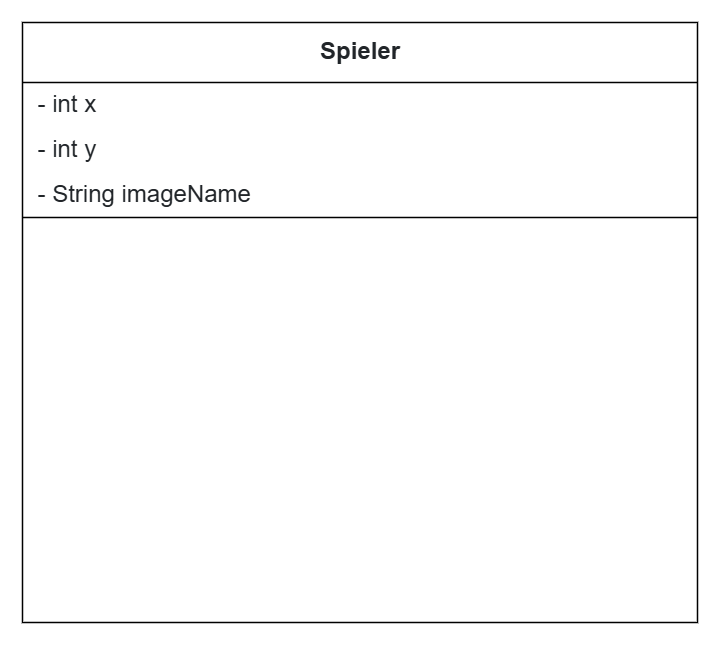
\includegraphics[width=1\linewidth]{_Aufgaben//BlocklyJava_Skript//img/H10_GetterSetter.png}

\begin{tikzpicture}
\begin{class}[text width=0.98\linewidth]{Spieler}{0 ,0}
\attribute{- int x}
\attribute{- int y}
\attribute{- String imagePath}
\operation{}
\operation{}
\operation{}
\operation{}
\operation{}
\operation{}
\operation{}
\operation{}
\end{class}
\end{tikzpicture}
}

\textbf{public void set}\emph{NameAttribut}\textbf{(}\emph{TypAttribut}~\textbf{wert)}\\

\Large \emphColA{Standard-Getter/-Setter} \large lesen bzw. schreiben den Wert des Attributs direkt (ohne Prüfung). Allgemein können Setter vor dem Schreiben den Parameter auf Gültigkeit prüfen oder modifizieren. 
}
